% ---- closed --------

\begin{figure}[!htb]
    \centering
    \begin{minipage}[b]{0.45\textwidth}
        \centering
        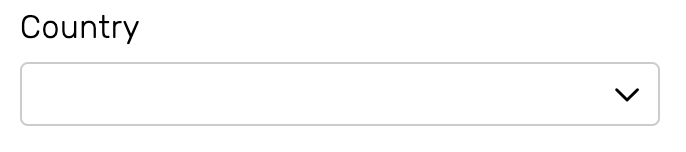
\includegraphics[width=0.8\textwidth]{closed.png}
        \caption{Geschlossene \codestyle{SelectComponent}}
        \label{img:closedNewComp}
    \end{minipage}
    \hfill
    \begin{minipage}[b]{0.45\textwidth}
        \centering
        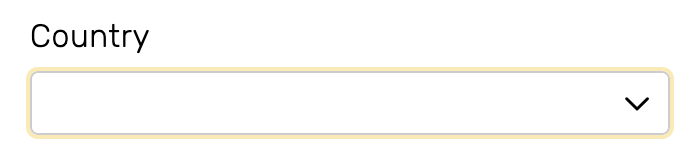
\includegraphics[width=0.8\textwidth]{closed.focused.png}
        \caption{Fokussierte \codestyle{SelectComponent}}
        \label{img:closedFocusedNewComp}
    \end{minipage}
\end{figure}

\begin{figure}[!htb]
    \centering
    \begin{minipage}[b]{0.45\textwidth}
        \centering
        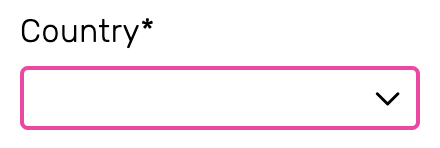
\includegraphics[width=0.8\textwidth]{closed.required.png}
        \caption{Required \codestyle{SelectComponent}}
        \label{img:closedRequiredNewComp}
    \end{minipage}
    \hfill
    \begin{minipage}[b]{0.45\textwidth}
        \centering
        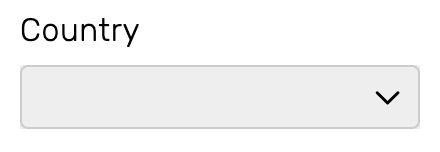
\includegraphics[width=0.8\textwidth]{closed.disabled.png}
        \caption{Disabled \codestyle{SelectComponent}}
        \label{img:closedDisabledNewComp}
    \end{minipage}
\end{figure}

\begin{figure}[!htb]
    \centering
    \begin{minipage}[b]{0.45\textwidth}
        \centering
        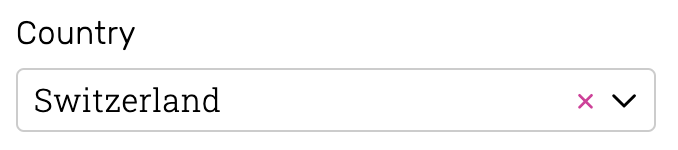
\includegraphics[width=0.8\textwidth]{closed.filled.png}
        \caption{Ausgefüllte \codestyle{SelectComponent}}
        \label{img:closedFilledNewComp}
    \end{minipage}
    \hfill
    \begin{minipage}[b]{0.45\textwidth}
        \centering
        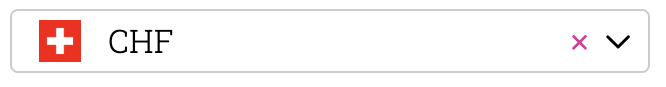
\includegraphics[width=0.8\textwidth]{closed.img.png}
        \caption{Ausgefüllte \codestyle{SelectComponent} mit Bild}
        \label{img:closedImgNewComp}
    \end{minipage}
\end{figure}

% ---- opened --------

\begin{figure}[!htb]
    \centering
    \begin{minipage}[b]{0.45\textwidth}
        \centering
        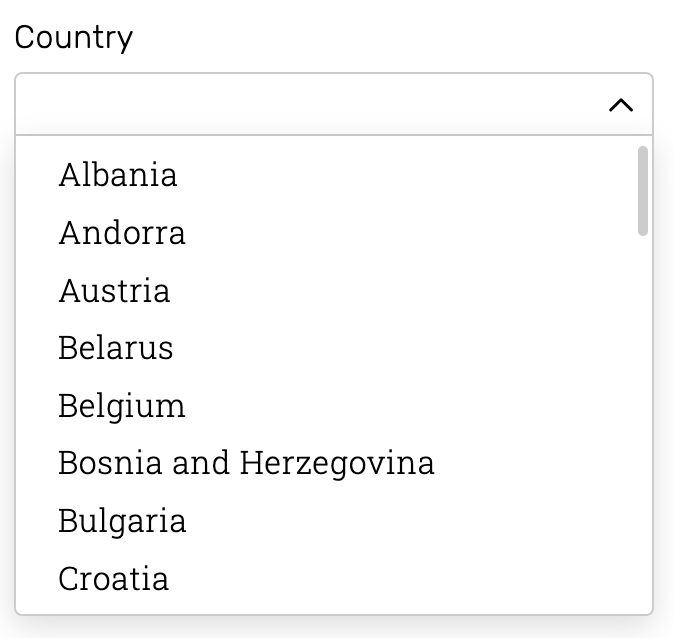
\includegraphics[width=0.8\textwidth]{opened.1col.png}
        \caption{Offene \codestyle{SelectComponent} - 1 Spalte}
        \label{img:openedOneColNewComp}
    \end{minipage}
    \hfill
    \begin{minipage}[b]{0.45\textwidth}
        \centering
        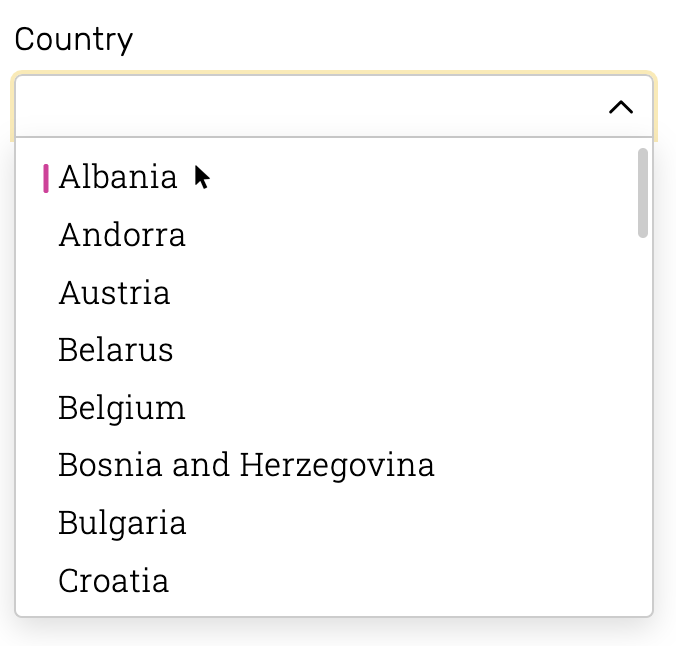
\includegraphics[width=0.8\textwidth]{opened.highlighted.png}
        \caption{Offene \codestyle{SelectComponent} mit Highlight}
        \label{img:openedHighlightedNewComp}
    \end{minipage}
\end{figure}

\begin{figure}[!htb]
    \centering
    \begin{minipage}[b]{0.45\textwidth}
        \centering
        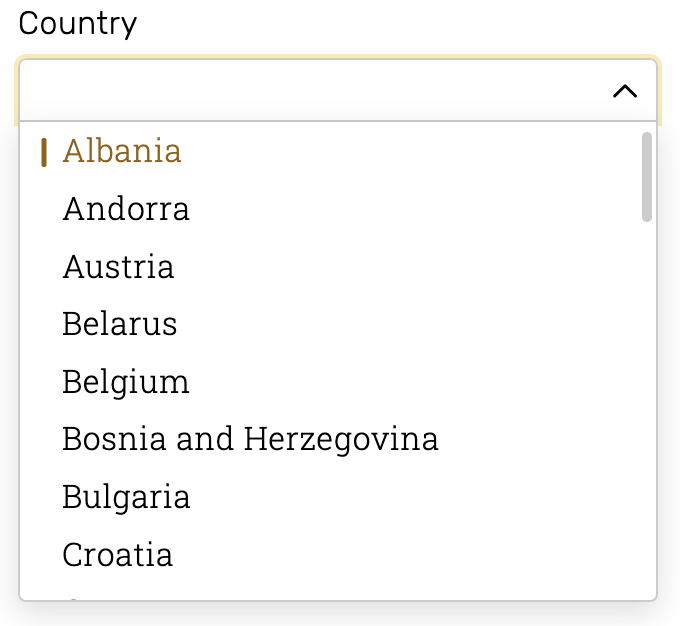
\includegraphics[width=0.8\textwidth]{opened.cursored.png}
        \caption{Offene \codestyle{SelectComponent} mit Cursor Position}
        \label{img:openedCursoredNewComp}
    \end{minipage}
    \hfill
    \begin{minipage}[b]{0.45\textwidth}
        \centering
        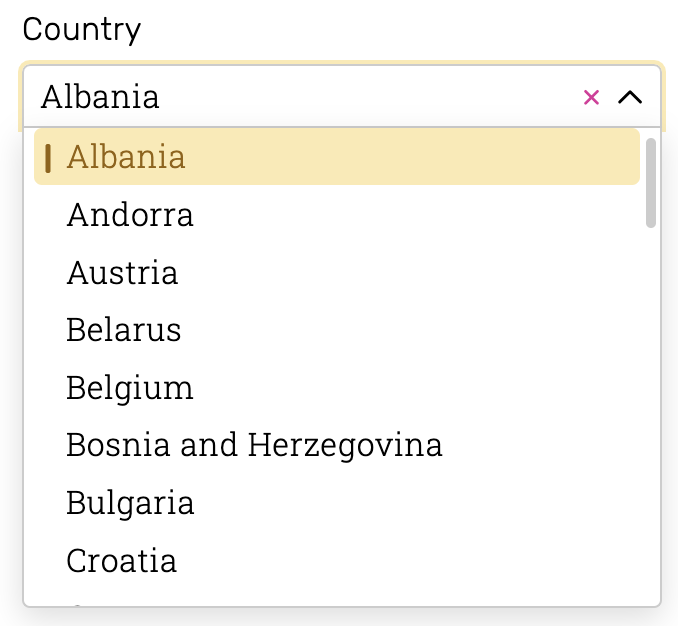
\includegraphics[width=0.8\textwidth]{opened.selected.png}
        \caption{Offene \codestyle{SelectComponent} mit Selektion}
        \label{img:openedSelectedNewComp}
    \end{minipage}
\end{figure}

\begin{figure}[!htb]
    \centering
    \begin{minipage}[b]{0.45\textwidth}
        \centering
        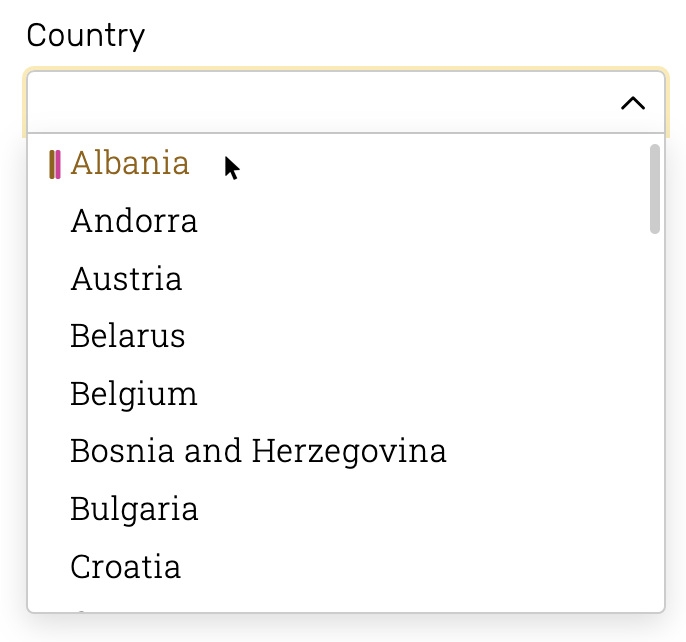
\includegraphics[width=0.8\textwidth]{opened.highlighted.cursored.png}
        \caption{Offene \codestyle{SelectComponent} mit Highlight \& Cursor Position}
        \label{img:openedHighlightedCursoredNewComp}
    \end{minipage}
    \hfill
    \begin{minipage}[b]{0.45\textwidth}
        \centering
        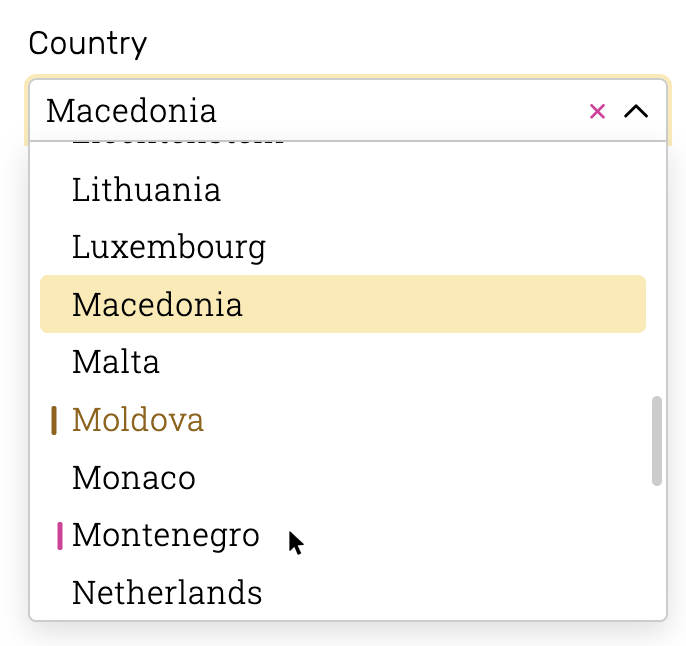
\includegraphics[width=0.8\textwidth]{opened.selected.cursored.highlighted.png}
        \caption{Offene \codestyle{SelectComponent} mit Highlight \& Cursor Position \& Selektion}
        \label{img:openedHighlightedCursoredSelectedNewComp}
    \end{minipage}
\end{figure}

\begin{figure}[!htb]
    \centering
    \begin{minipage}[b]{0.45\textwidth}
        \centering
        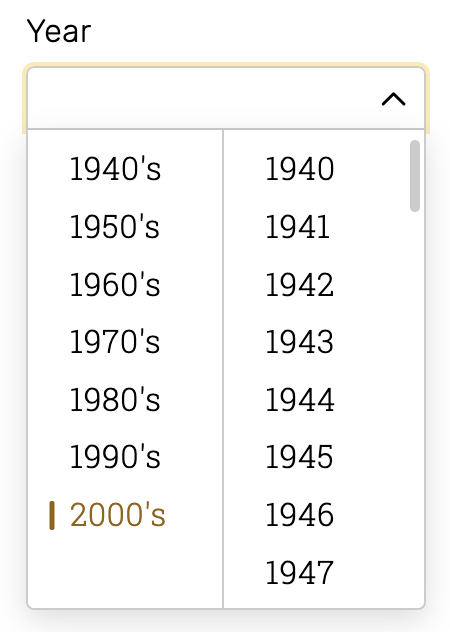
\includegraphics[width=0.8\textwidth]{opened.2col.png}
        \caption{Offene \codestyle{SelectComponent} - 2 Spalten}
        \label{img:openedTwoColNewComp}
    \end{minipage}
    \hfill
    \begin{minipage}[b]{0.45\textwidth}
        \centering
        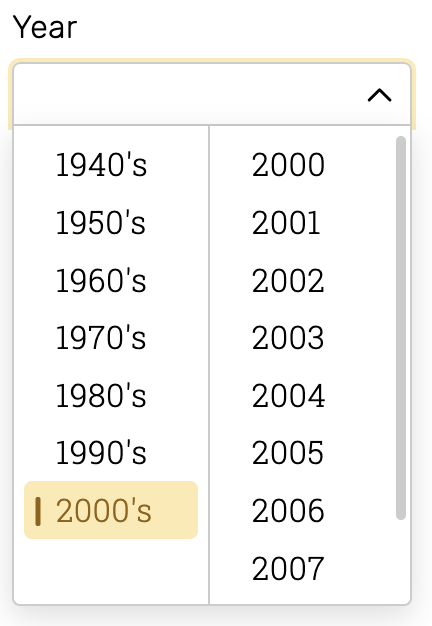
\includegraphics[width=0.8\textwidth]{opened.2col.categoried.png}
        \caption{Offene \codestyle{SelectComponent} mit Kategorie-Selektion}
        \label{img:openedTwoColCatNewComp}
    \end{minipage}
\end{figure}

\begin{figure}[!htb]
    \centering
    \begin{minipage}[b]{0.45\textwidth}
        \centering
        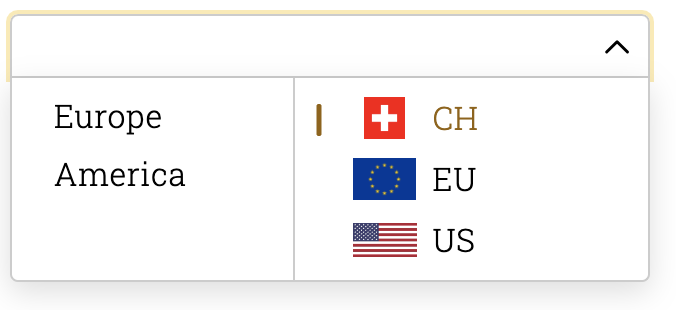
\includegraphics[width=0.8\textwidth]{opened.img.png}
        \caption{Offene \codestyle{SelectComponent} mit Bilder}
        \label{img:openedTwoColImgNewComp}
    \end{minipage}
    \hfill
    \begin{minipage}[b]{0.45\textwidth}
        \centering
        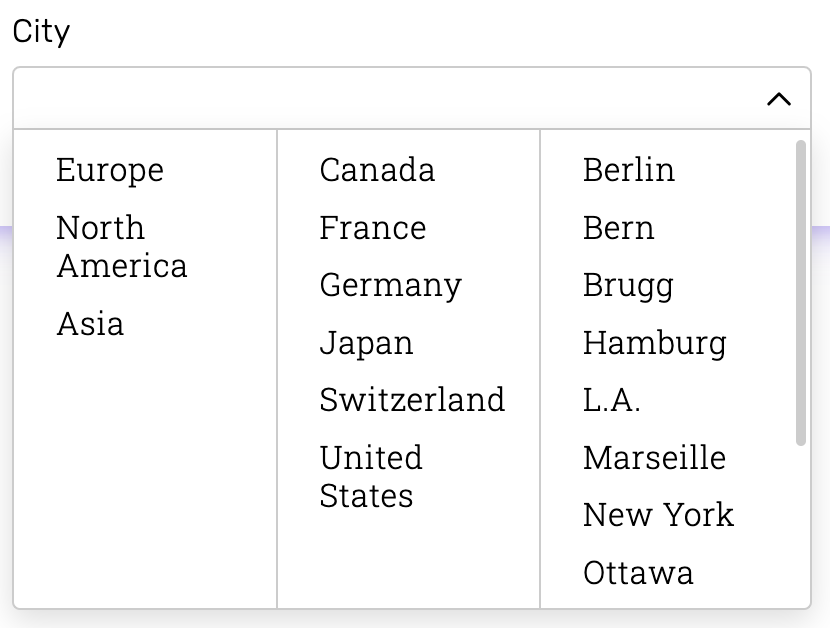
\includegraphics[width=0.8\textwidth]{opened.3col.png}
        \caption{Offene \codestyle{SelectComponent} - 3 Spalten}
        \label{img:openedThreeColNewComp}
    \end{minipage}
\end{figure}

\begin{figure}[!htb]
    \centering
    \begin{minipage}[b]{0.45\textwidth}
        \centering
        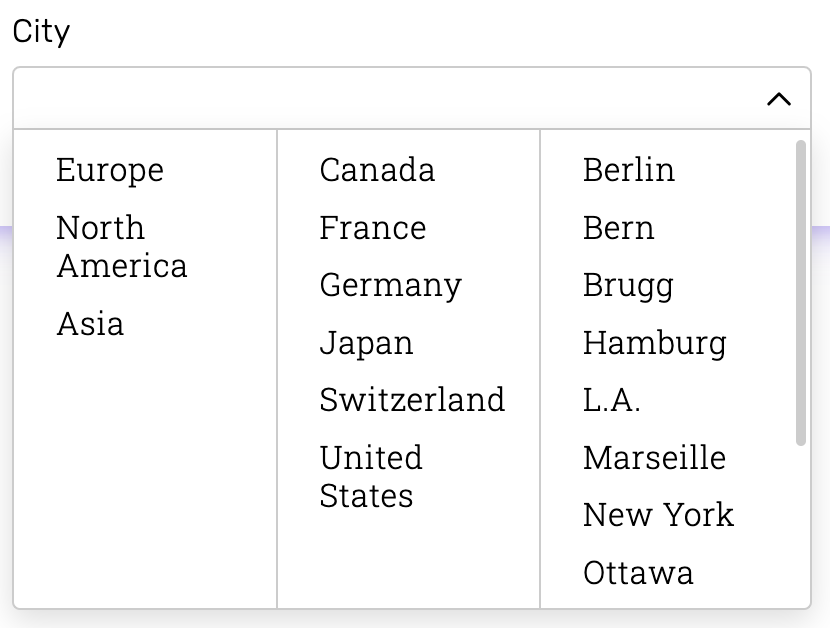
\includegraphics[width=0.8\textwidth]{opened.3col.png}
        \caption{Offene \codestyle{SelectComponent} mit Kategorie-Selektion}
        \label{img:openedThreeColCatNewComp}
    \end{minipage}
    \hfill
    \begin{minipage}[b]{0.45\textwidth}
        \centering
        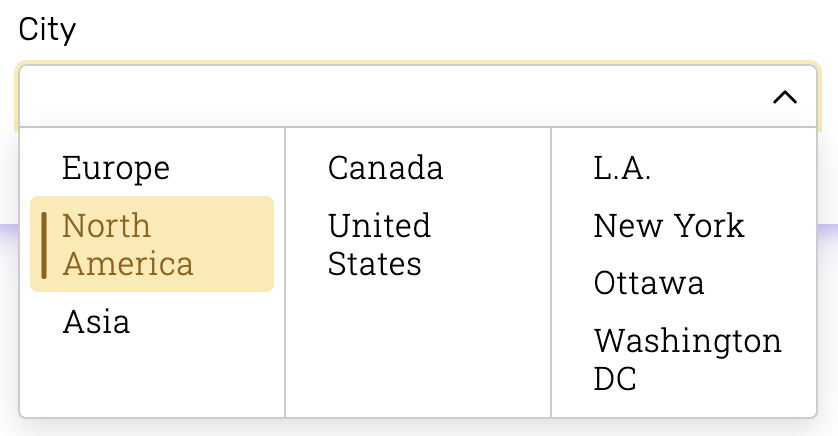
\includegraphics[width=0.8\textwidth]{opened.3col.categoried.png}
        \caption{Offene \codestyle{SelectComponent} mit Kategorie- \& Subkategorie-Selektion}
        \label{img:openedThreeColCatSubcatNewComp}
    \end{minipage}
\end{figure}
